\section{Combinazione agli SLE rara}
Secondo la $[2.5.2]$ della normativa di riferimento, la combinazione caratteristica per gli SLE irreversibili è così definita
\[
	G_1 + G_2 + Q_{1k} + \psi_{02}\cdot Q_{2k} + \psi_{03}\cdot Q_{3k} + \dots
\]

Nella combinazione caratteristica, al contrario della fondamentale, non sono presenti i coefficienti di sicurezza $\gamma$, ma solamente i coefficienti di combinazione $\psi$. Si ha, comunque, la necessità di considerare diverse combinazioni di carichi per valutare i valori massimo e minimo. In questa sezione, per non dilungarsi troppo, ripetendo quanto fatto nei paragrafi precedenti, si tralasceranno le combinazioni che non danno il contributo massimo o minimo desiderato. Verranno, perciò, trascritti solo i valori di riferimento, tenendo presente che le altre combinazioni sono comunque presenti nel foglio di calcolo.

\subsection{Calcolo delle azioni massime e minime}
\subsubsection*{Tratto $P13\div P16$}
\begin{equation*}
	\begin{cases}
		Q_{1,max} &= 8.00+11.52+3.75 + 11.55+7.98+9.20 + 15.01 + 0.7\cdot(7.50+14.40) + 0.6\cdot0.5\\
		&= 82.64\,\dfrac{kN}{m}\\\\
		Q_{1,min} &= 8.00+11.52+3.75 + 11.55+7.98+9.20 + 0.5\cdot8.68 +7.50 + 0.7\cdot14.40 + 0.6\cdot0.5\\
		&= 74.18\,\dfrac{kN}{m}
	\end{cases}
\end{equation*}

Il massimo deriva dalla combinazione con neve principale mentre il minimo con la combinazione con la categoria B2 del solaio interno principale.

\subsubsection*{Tratto $P16\div P17$}
\begin{equation*}
	\begin{cases}
		Q_{2,max} &= 8.00+6.72+3.75 + 11.55+4.65+9.20 + 10.30 + 0.7\cdot(7.50+8.40) + 0.6\cdot0.3\\
		&= 65.48\,\dfrac{kN}{m}\\\\
		Q_{2,min} &= 8.00+6.72+3.75 + 11.55+4.65+9.20 + 0.5\cdot 5.06 + 7.50 + 0.7\cdot 8.40 + 0.6\cdot0.3\\
		&= 59.96\,\dfrac{kN}{m}
	\end{cases}
\end{equation*}
rispettivamente per il carico da neve principale la categoria B2 principale.

\subsubsection*{Tratto $P17$ - vano scala}
\begin{equation*}
	\begin{cases}
		Q_{3,max} &= 8.00+3.20+3.75 + 11.55+2.215+9.20 + 4.17 + 0.7\cdot(7.50+4.00) + 0.6\cdot0.138\\
		&= 50.22\,\dfrac{kN}{m}\\\\
		Q_{3,min} &= 8.00+3.20+3.75 + 11.55+2.215+9.20 + 0.5\cdot2.41 + 4+ 0.7\cdot7.50 + 0.6\cdot0.138\\
		&= 48.45\,\dfrac{kN}{m}
	\end{cases}
\end{equation*}

Mentre il massimo ricade sempre nella combinazione con l'azione della neve principale, il minimo valore, poiché il solaio è ordito in maniera parallela alla trave e perciò la lunghezza di influenza è decisamente minore e pari a $1\,m$, è attribuito al sovraccarico di categoria della terrazza.

Sostitendo i valori nelle otto combinazioni e sovrapponendole, si ottiene la figura~\ref{fig:bendingMomentComparison_sleRara}, da cui deriva il diagramma dell'inviluppo di figura~\ref{fig:bendingMomentEnvelope_sleRara}

\begin{figure}
	\centering
	
	\subfloat[\emph{Confronto delle combinazioni}]{\label{fig:bendingMomentComparison_sleRara}
	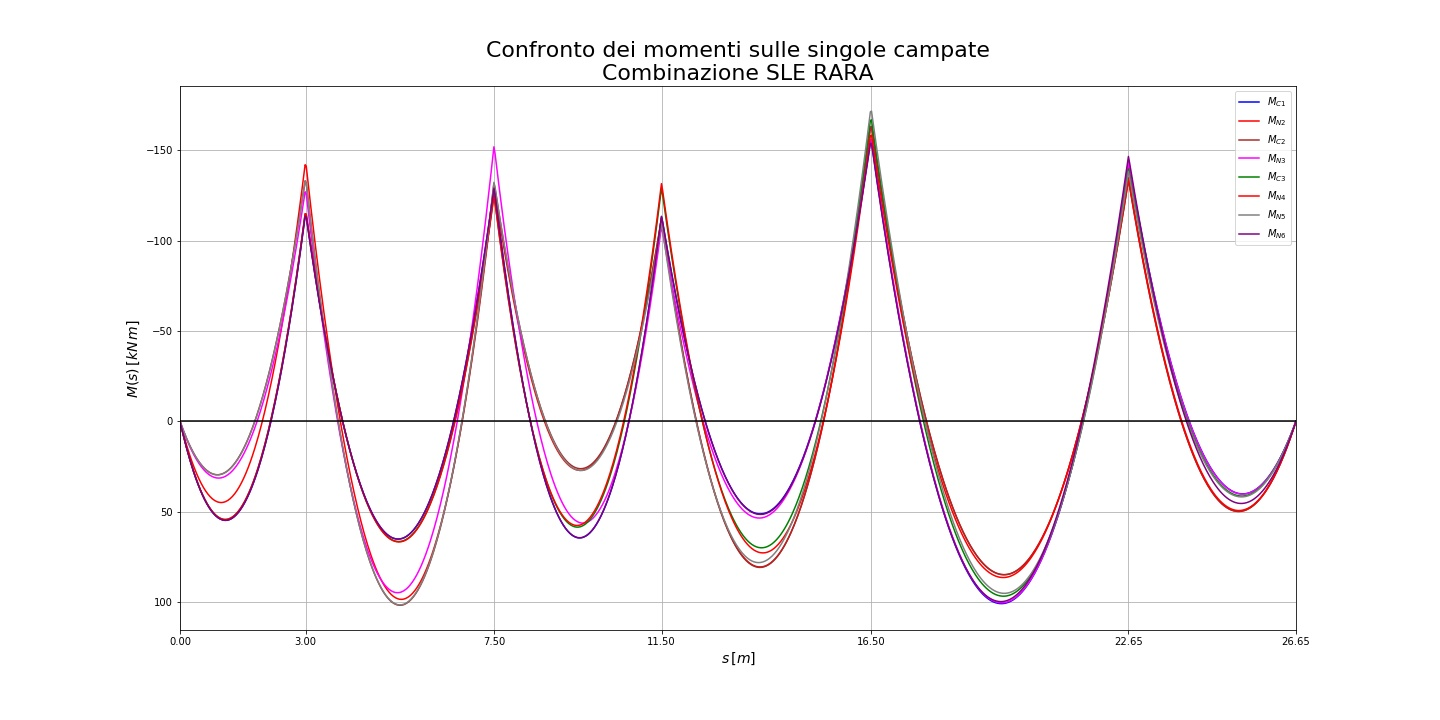
\includegraphics[width=\textwidth]{../../export/img/bendingMomentComparison_sleRara}}\\
	\subfloat[\emph{Inviluppo dei momenti flettenti}]{\label{fig:bendingMomentEnvelope_sleRara}
	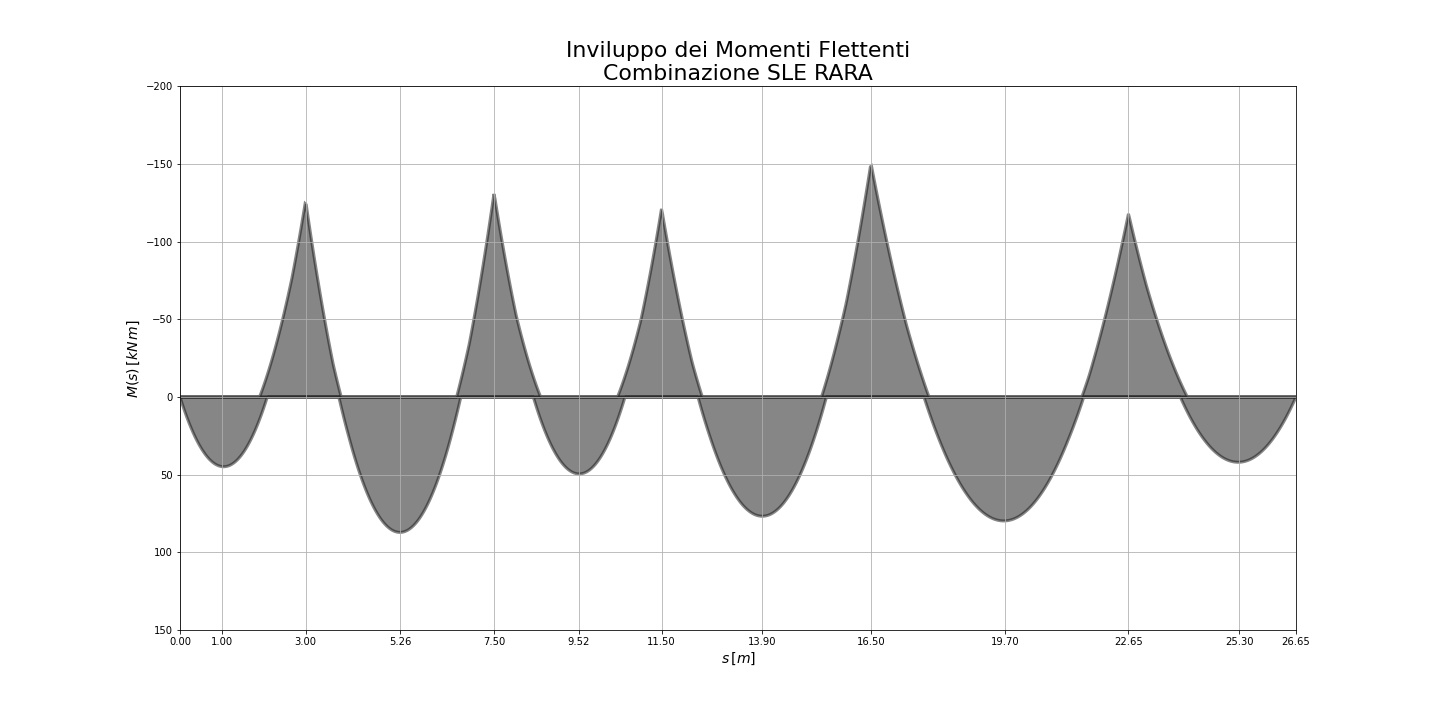
\includegraphics[width=\textwidth]{../../export/img/bendingMomentEnvelope_sleRara}}
	\caption{Diagramma del momento flettente per la combinazione SLE rara}
	\label{fig:bendingMoment_sleRara}
\end{figure}

La tabella~\ref{tab:max_min_bendingMomentEnvelope_sleRara} raccoglie i valori massimi e minimi dei momenti.

\begin{table}
  	\centering
  	\caption{Valori massimi e minimi dell'inviluppo dei momenti}
  	\label{tab:max_min_bendingMomentEnvelope_sleRara}
  	\begin{tabular}{lcccr}
		\toprule
		& $M_{Ed}^+\,[kN\,m]$ & $s_{max}\,[m]$ & $M_{Ed}^-\,[kN\,m]$ & $s_{min}\,[m]$ \\
		Sezione &             &          &             &          \\
		\midrule
		C1      &     44.9674 &        1 &         NaN &      NaN \\
N2      &         NaN &      NaN &    -124.213 &        3 \\
C2      &     86.7868 &     5.26 &           0 &      NaN \\
N3      &         NaN &      NaN &    -131.621 &      7.5 \\
C3      &     50.7991 &     9.55 &           0 &      NaN \\
N4      &         NaN &      NaN &    -117.001 &     11.5 \\
C4      &     72.2195 &    13.85 &           0 &      NaN \\
N5      &         NaN &      NaN &    -159.946 &     16.5 \\
C5      &     93.2124 &     19.6 &           0 &      NaN \\
N6      &         NaN &      NaN &    -137.047 &    22.65 \\
C6      &     45.7521 &       25 &         NaN &      NaN \\
\bottomrule
	\end{tabular}
  \end{table}
  
\begin{figure}
	\centering
	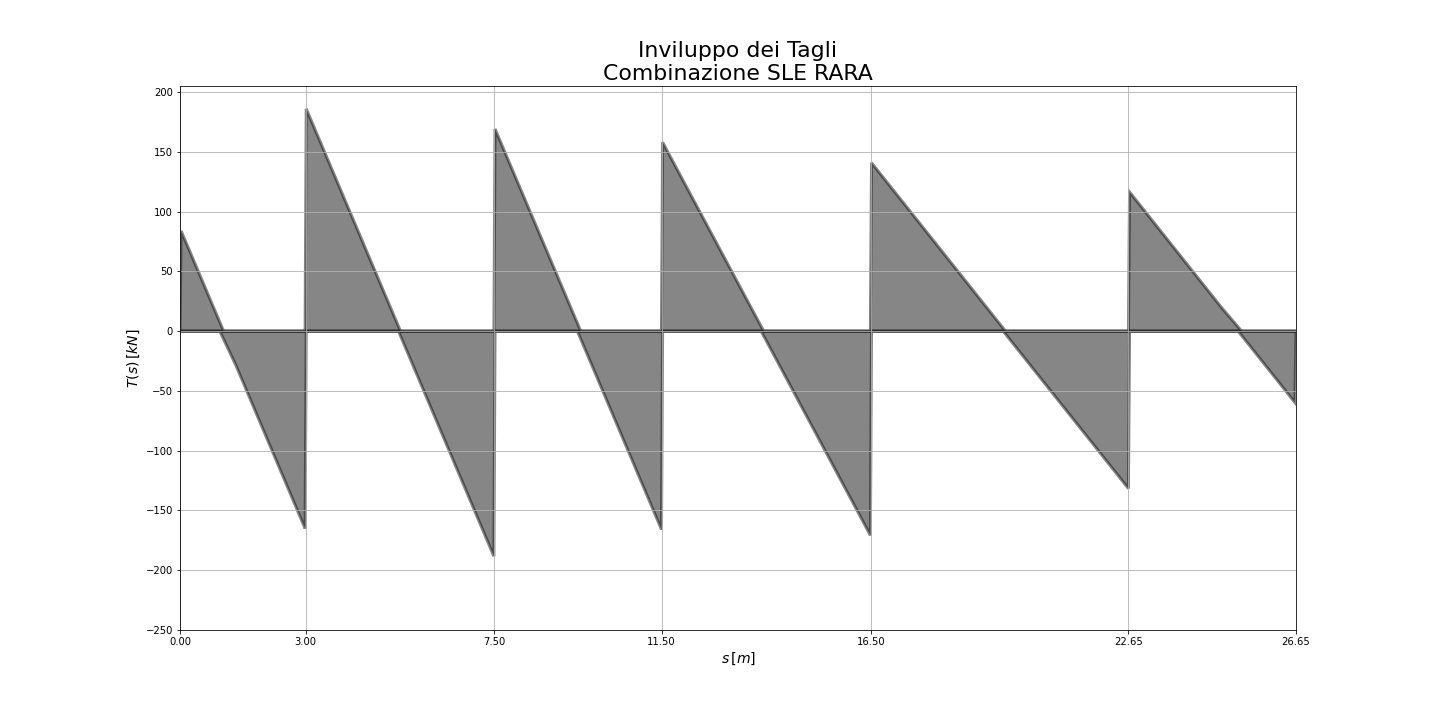
\includegraphics[width=\textwidth]{../../export/img/shearEnvelope_sleRara}
	\caption{Diagramma dell'inviluppo dei tagli - Combinazone SLE rara}
\end{figure}

\begin{table}
  	\centering
  	\caption{Valori massimi e minimi dell'inviluppo dei tagli}
  	\label{tab:shearEnvelope_sleRara}
  	\begin{tabular}{lcccr}
		\toprule
		& $T_{Ed}^+\,[kN]$ & $s_{max}\,[m]$ & $T_{Ed}^-\,[kN]$ & $s_{min}\,[m]$ \\
		Sezione &             &          &             &          \\
		\midrule
N1      &    84.006 &        0 &         0 &        0 \\
N2      &   185.787 &        3 &  -165.029 &        3 \\
N3      &   170.316 &      7.5 &  -188.546 &      7.5 \\
N4      &   154.466 &     11.5 &  -164.588 &     11.5 \\
N5      &   158.492 &     16.5 &  -173.737 &     16.5 \\
N6      &    133.49 &    22.65 &   -151.89 &    22.65 \\
N7      &         0 &    26.65 &  -66.4499 &    26.65 \\
		\bottomrule
	\end{tabular}
  \end{table}

\cleardoublepage

